% LTeX: language=en-US

\begin{frame}{Motivation}
  \begin{witemize}
    \item Since Dynare 5, Method of Moments toolbox that provides functionality to
    estimate parameters by
    \begin{enumerate}
      \item Simulated Method of Moments (SMM) up to any perturbation
            approximation order (with or without pruning)
      \item Generalized Method of Moments (GMM) up to 3rd-order pruned
            perturbation approximation
    \end{enumerate}
    \item Toolbox is inspired by replication codes accompanied to \textcite{AndreasenEtal2018,BornPfeifer2014JME,Mutschler2018}
    \item Dynare 6: support for (Bayesian) impulse response function matching
    \item Inspired by \textcite{CEE2005} and \textcite{ChristianoTrabandtWalentin2010}
  \end{witemize}

\end{frame}


\section[Moments]{Computing moments in Dynare}
%\renewcommand{\Source}{Maddison Data Set}
\begin{frame}{Dynare's stochastic simulation framework}

  \begin{witemize}
    \item General DSGE model with shocks $u_t$, variables $y_t$, structural parameters $\theta$, and perturbation parameter $\sigma$ can be written as
    \begin{align}
      0   & =E_t f(y_{t+1}, y_t, y_{t-1}, u_t | \theta)                                     \\
      u_t & = \sigma \eta_t, \quad \text{with} \quad \eta_t \overset{iid}{\sim} N(0,\Sigma)
    \end{align}
    \item Note that
    \begin{align}
      E[u_t]      & = 0                          \\
      E[u_t u_t'] & = \Sigma_u = \sigma^2 \Sigma
    \end{align}

    \item Sidenote: shock distributions other than Gaussian are not (yet) supported by Dynare
    \item The solution, i.e.\ the policy functions take the generic form
    \begin{align}
      y_t = g(x_{t-1}, u_t | \theta)
    \end{align}
  \end{witemize}

\end{frame}

\begin{frame}{DSGE solution: perturbation}
  \begin{witemize}
    \item Perturbation solution involves taking a Taylor-approximation around the non-stochastic steady-state (where $y_t$ are all endogenous and $x_t$ are states)
    \item Solution at arbitrary order then takes the form:
    \begin{equation}
      \begin{split}
        {y_t} = & \bar y + {g_x}({x_{t - 1}} - \bar x) + {g_u}{u_t}                                                                                                                                     \\
                & + \frac{1}{2}[{g_{xx}}({x_{t - 1}} - \bar x) \otimes ({x_{t - 1}} - \bar x) + 2{g_{xu}}({x_{t - 1}} \otimes {u_t}) + {g_{uu}}({u_t} \otimes {u_t}) + {g_{\sigma \sigma }}{\sigma ^2}] \\
                & + \frac{1}{6}[\ldots]                                                                                                                                                                 \\
                & + \ldots
      \end{split}
    \end{equation}
  \end{witemize}

\end{frame}

\begin{frame}{How to compute moments?}
  \begin{witemize}
    \item Want to pin down some of the parameters in $\theta$ by some form of moment matching
    \item Two ways of computing moments:
    \begin{enumerate}
      \item Via simulation (\texttt{periods} option): Use approximated policy function to simulate data and compute the mean, covariance, auto-covariance, skewness, kurtosis, \ldots
      \item Use theoretical expressions based on state space representation\\
            $\rightarrow$ did that e.g.\ for the Kalman filter initialization
    \end{enumerate}
  \end{witemize}
\end{frame}

\begin{frame}{First-order approximation and moments}
  \begin{itemize}
    \item Consider first order approximation of policy rule:
          \begin{align}
            y_t = \bar{y} + g_x(x_{t-1} - \bar{x}) + g_u u_t, \\
            x_t = \bar{x} + h_x(x_{t-1} - \bar{x}) + h_u u_t
          \end{align}
    \item Unconditional first and second moments are
          \begin{align}
            E\left[y_t\right]      & = \mu_y = \bar{y}                                                                                             \\
            E\left[x_t\right]      & = \mu_x = \bar{x}                                                                                             \\
            \Sigma_y\left(0\right) & = E\left[(y_t - \bar{y})(y_t - \bar{y})'\right] = g_{x} \Sigma_x\left(0\right)g_{x}' + g_u \Sigma_u g_u'      \\
            \Sigma_x\left(0\right) & = E\left[(x_t - \bar{x})(x_t - \bar{x})'\right] = h_{x} \Sigma_x\left(0\right)h_{x}' + h_u \Sigma_u h_u' \: ,
          \end{align}
          where $\Sigma_x(0)$ is fixed point of Lyapunov equation
    \item Result allows computing auto-covariogram at lag $j$: \(\Sigma_x(j)\) and \(\Sigma_y(j)\)
  \end{itemize}
\end{frame}


\begin{frame}{Higher-order approximation: the challenge}

  \begin{witemize}
    \item Perturbation approximations are polynomials and thus have unavoidable oscillations
    \item Higher order perturbation policy functions do not inherit properties like monotonicity and convexity from the true policy functions
    \item Moreover, no way to control where such oscillations occur
    \item[$\rightarrow$] could occur close to steady state
    \item Consider a univariate second-order example (setting uncertainty correction $\frac{1}{2}g_{\sigma\sigma}\sigma^2=0$) with policy function:
    \begin{equation}
      x_t = g_x x_{t-1} + g_{xx} x_{t-1}^2 + g_u u_t, \quad |g_x| < 1, \quad g_{xx} > 0
    \end{equation}

    \item $|g_x| < 1$ ensures that first-order approximation is stable and unique.

    \item Second-order approximation has two fixed-points: $\bar{x} = 0$ and $\bar{x} = \frac{1 - g_x}{g_{xx}}$

    $\Rightarrow$ Once the model passes the second fixed point it will explode

  \end{witemize}

\end{frame}


\begin{frame}{Example from \textcite{DenHaanDeWind2012}}
  \begin{columns}
    \begin{column}{0.5\textwidth}
      \begin{figure}
        \centering
        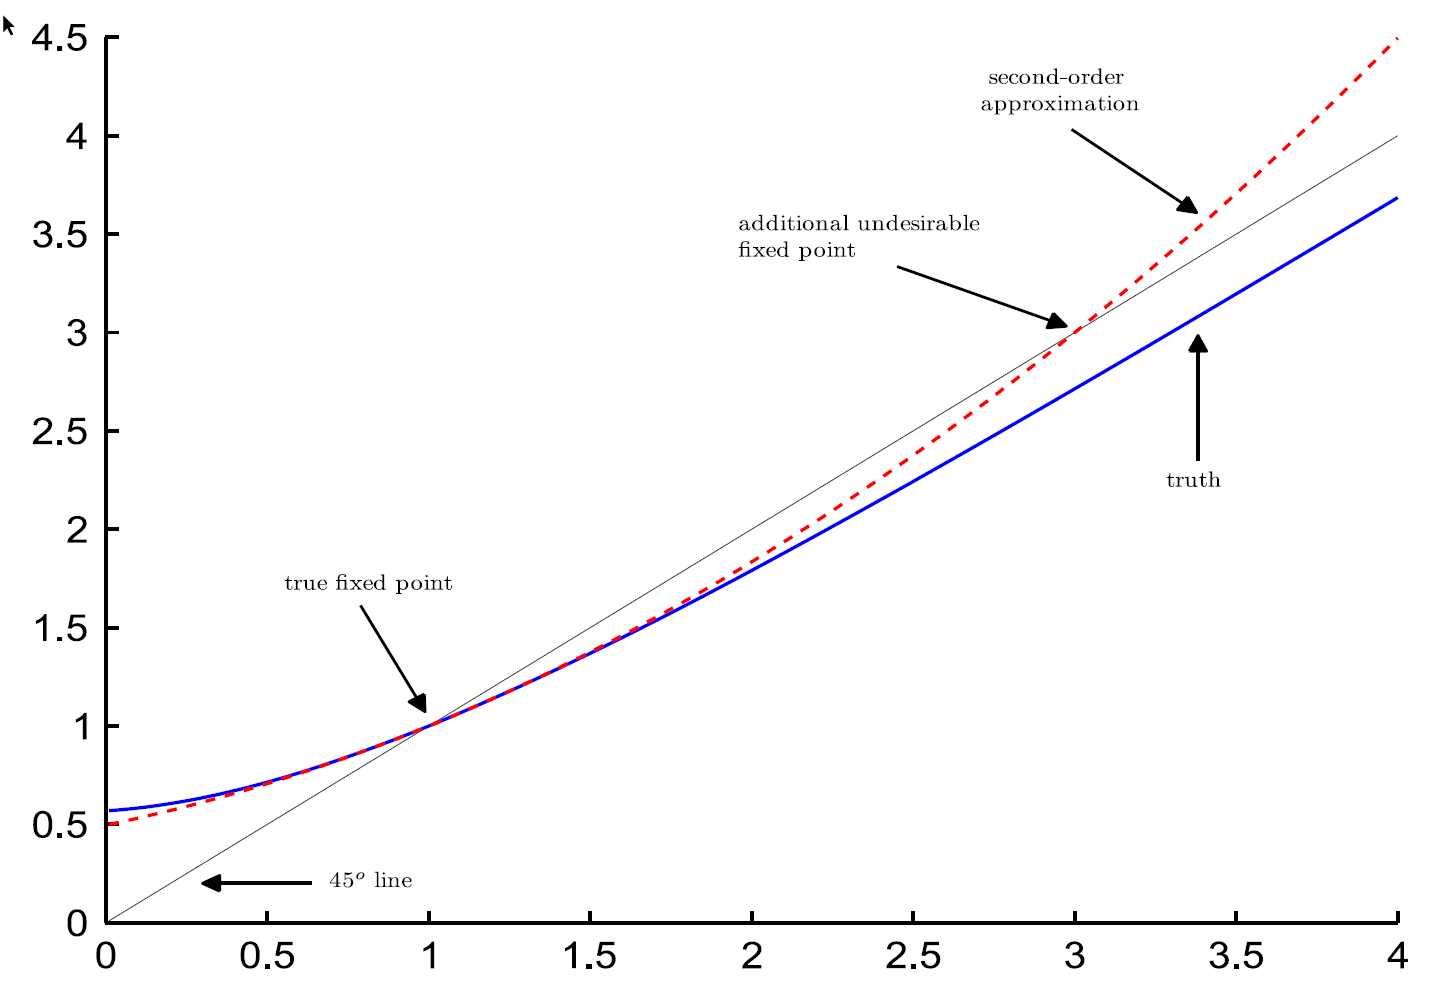
\includegraphics[width=\textwidth]{Figures/Den_Haan_DeWind_2012}
      \end{figure}
    \end{column}
    \begin{column}{0.5\textwidth}
      \begin{witemize}
        \item Consider policy function with unique fixed point at 1 and globally stable dynamics
        \begin{equation}
          x_t = \frac{0.9}{e}+x_{t-1}+0.9 e^{-x_{t-1}}
        \end{equation}
        \item Second-order approximation inherits
        \begin{itemize}
          \item increasing in $x_{t-1}$
          \item strictly convex $x_{t-1}$
          \item local stability as slope at steady state is smaller than 1
        \end{itemize}
        \item Such a polynomial must have second fixed point and globally unstable dynamics\\
        $\rightarrow$ explosive for large shocks
      \end{witemize}
    \end{column}
  \end{columns}
\end{frame}

\begin{frame}{A slightly different take}
  \begin{witemize}
    \item As first noted in \textcite{KKSS2008}, higher order perturbation solutions tend to explode due to the accumulation of terms of increasing order
    \item For example, in second order approximated solution, quadratic term at time $t$ will be raised to the power of two in the quadratic term at $t+1$
    \item Resulting in quartic term will become a term of order 8 at $t+2$ and so on
  \end{witemize}
\end{frame}

\begin{frame}{Solving the explosiveness of higher-order approximations}
  \begin{witemize}
    \item Possibility of explosive behavior in higher-order approximations\\
    $\rightarrow$ Model may not be stationary or does not have an ergodic probability distribution
    \item Solution: \highlight{Pruning}
    \begin{witemize}
      \item Leave out terms in solution that have higher-order effects than the approximation order\\
      $\rightarrow$ squaring second order term one period later results in term of fourth order
      \item \textcite{KKSS2008} and \textcite{AndreasenEtal2018}: pruned state space is stationary and ergodic (conditional on regularity conditions for the shocks)
      \item \textcite{LombardoUhlig2018} or \textcite{LanMeyerGohde2013pruning} provide theoretical foundation for this seemingly ad-hoc procedure
    \end{witemize}

  \end{witemize}
\end{frame}



\begin{frame}{Pruning for univariate example}

  \begin{itemize}
    \item Decompose state vector into 1st- and 2nd-order effects
          \begin{equation}
            x_t = x_t^f + x_t^s = g_{x}x_{t-1}^f  + g_{x}x_{t-1}^s + g_{xx}(x_{t-1}^f)^2 + 2g_{xx}x_{t-1}^f x_{t-1}^s + g_{xx}(x_{t-1}^s)^2 + g_{u}u_t
          \end{equation}

    \item Stable solution: Prune terms that contain $x_t^f x_t^s$ and $(x_t^s)^2$ to get law of motions:
          \begin{align}
            x_t^f & = g_{x}x_{t-1}^f + g_{u}u_t            \\
            x_t^s & = g_{x}x_{t-1}^s + g_{xx}(x_{t-1}^f)^2
          \end{align}
          where
          \begin{equation}
            \left(x_t^f\right)^2 = g_{xx}^2 \left(x_{t-1}^f\right)^2 + 2g_{xx}g_{u}x_{t-1}^f u_t + g_{u}^2 u_t^2
          \end{equation}
  \end{itemize}
\end{frame}



\begin{frame}{Univariate example}
  \begin{itemize}
    \item Pruned solution can be compactly rewritten as a stable state-space system

          \begin{equation}
            \underbrace{\begin{bmatrix}
                x_t^f \\
                x_t^s \\
                (x_t^f)^2
              \end{bmatrix}}_{z_t} = \underbrace{\begin{bmatrix}
                g_x & 0   & 0        \\
                0   & g_x & g_{xx}   \\
                0   & 0   & g_{xx}^2
              \end{bmatrix}}_A
            \underbrace{\begin{bmatrix}
                x_{t-1}^f \\
                x_{t-1}^s \\
                (x_{t-1}^f)^2
              \end{bmatrix}}_{z_{t-1}} +  \underbrace{\begin{bmatrix}
                g_u & 0       & 0     \\
                0   & 0       & 0     \\
                0   & 2g_xg_u & g_u^2
              \end{bmatrix}}_B\underbrace{\begin{bmatrix}
                u_t           \\
                x_{t-1}^f u_t \\
                u_t^2 - \sigma_u^2
              \end{bmatrix}}_{\xi_t} + \underbrace{\begin{bmatrix}
                0 \\
                0 \\
                g_u^2 \sigma_u^2
              \end{bmatrix}}_c
          \end{equation}

    \item Formulation assures that $\xi_t$ is mean 0
    \item Note: Even if $u_t$ is Gaussian, $\xi_t$ is not!\\
          $\rightarrow$ Higher-order statistics (HOS) may contain additional information for estimation
  \end{itemize}
\end{frame}


\begin{frame}{Pruned state space system}
  \begin{witemize}
    \item Given an extended state vector \( z_t \) and an extended vector of innovations \( \xi_t \), the pruned perturbation solution of a DSGE model can be rewritten as a linear time-invariant state-space system for any approximation order \parencite{AndreasenEtal2018}:
    \begin{align}
      z_t & = c + A z_{t-1} + B \xi_t           \\
      y_t & = \bar{y} + d + C z_{t-1} + D \xi_t
    \end{align}
    \item Remember: usually non-Gaussian!

    \item Straightforward (but tedious) to compute moments (very similar to first-order)

  \end{witemize}

\end{frame}

\begin{frame}{A note on the state space}
  \begin{witemize}
    \item As can be seen, we now need to keep track of all components of the state variables instead of the just their sum, i.e.\ the original state\\
    $\rightarrow$ pruning introduces additional state variables not part of the original state space
    \item $n$th order pruned solution does not deliver exact solution, even if the true policy function is an $n$th order polynomial (but raising approximation order alleviates this)
    \item Fortunately, it seems as if the accuracy problems occur mostly outside the ergodic set of many economic problems
    \item However: there is no guarantee that this transfers to other applications
    \item Needing to keep track of the individual terms also reintroduces curse of dimensionality
  \end{witemize}
\end{frame}

\section{Method of Moments}


\begin{frame}{Calibration}

  \begin{witemize}
    \item Calibration: choose parameter values to match model moments to the data moments\\
    $\rightarrow$ usually one-to-one mapping
    \item Dates back to at least \textcite{KydlandPrescott1982}, who used it to evaluate the performance of the RBC model
    \item Original idea: choose parameter values to make the model consistent with growth observations, but judge model's performance to explain business cycles\\
    $\rightarrow$ don't use same data for calibration and evaluation
  \end{witemize}

\end{frame}


\begin{frame}{Moment matching: basic idea}

  \begin{witemize}
    \item Calibration often too restrictive:
    \begin{itemize}
      \item no straightforward one-to-one mapping\\
      \item parameters not identified by growth observations
      \item unclear which targets to match
      \item efficiency concerns when not jointly setting parameters
      \item How to quantify uncertainty?
    \end{itemize}
    \item Solution: formulate formal estimation problem: try to minimize the distance between model moments and data moments
    \begin{enumerate}
      \item Simulated Method of Moments: model moments are computed via simulations
      \item Generalized Method of Moments: model moments are computed theoretically
      \item IRF matching: model IRFs are matched to empirical IRFs
    \end{enumerate}
  \end{witemize}

\end{frame}


\subsection{SMM}

\begin{frame}{Simulated Method of Moments: notation}

  \begin{witemize}
    \item $m_t$: vector of empirical observations with $T$ observations on variables whose moments
    \begin{equation}
      \frac{1}{T} \sum_{t=1}^{T} m_t
    \end{equation}
    are of interest (e.g.\ $ y_t, c_t, y_{t}y_{t-1}, y_t^3 $)
    \item $m_i(\theta)$: model counterpart of $m$, computed on basis of $T'=\tau T$ observations of artificial data generated using parameter values $\theta $\\
    $\rightarrow$ multiple $\tau$ of empirical data
    \item $W$: positive definite weighting matrix (if you have more moments than parameters)

  \end{witemize}
\end{frame}

\begin{frame}{Choice of the weighting matrix}
  \begin{itemize}
    \item Any positive definite weighting matrix works
    \item But: there is only one optimal weighting matrix $W^{opt}$ minimizing the asymptotic variance of the estimator, i.e.\ having the tightest bands: the inverse of the long-run covariance matrix of the moments\\
          $\rightarrow$ weights moments with their precision (similar to GLS)
    \item Problem: long-run variance is unknown (depends on true parameter vector) and needs to be estimated using plug-in estimator\\
          $\rightarrow$ usually a \textcite{NeweyWest1987}-type estimator with a Bartlett kernel
    \item Popular approach: two stage/iterated GMM/SMM
          \begin{enumerate}
            \item use non-optimal, typically diagonal weighting matrix in first stage\\
                  $\rightarrow$ consistent but inefficient parameter estimate
            \item Use parameter estimate to recompute long-run variance of moments\\
                  $\rightarrow$ asymptotically efficient
          \end{enumerate}
  \end{itemize}
\end{frame}



\begin{frame}{Simulated Method of Moments estimator}
  \begin{itemize}
    \item Goal: minimize distance $G(\theta)$ between empirical and model simulated moments:
          \begin{equation}
            G(\theta) = \frac{1}{T} \sum_{t=1}^{T} m_t - \frac{1}{\tau T} \sum_{i}^{\tau T} m_i(\theta)
          \end{equation}

    \item SMM estimator $\hat{\theta}_{\text{SMM}}$ is the value that minimizes

          \begin{equation}
            {\hat \theta _{SMM}} = \mathop {\text{argmin}}\limits_\theta  \left( {G\left( \theta  \right)} \right)'WG\left( \theta  \right)
          \end{equation}

    \item Dynare provides rich suite of numerical tools to solve this minimization problem
  \end{itemize}
\end{frame}


\begin{frame}{Statistical properties of SMM estimator}
  \begin{itemize}
    \item Under regularity conditions in \textcite{DuffieSingleton1993} and when using the optimal weighting matrix $W^{opt}$:
          \begin{equation}
            \sqrt{T} (\hat{\theta}_{\text{SMM}} - \theta) \rightarrow N \left( 0, (1 + 1/\tau)(D'W^{opt}D)^{-1} \right)
          \end{equation}
    \item $ W $ is computed using a \textcite{NeweyWest1987}-type estimator with a Bartlett kernel
    \item Sandwich matrix

          \begin{equation}
            D = E \left[ \frac{\partial m_i(\theta)}{\partial \theta} \right]
          \end{equation}

          \begin{itemize}
            \item must be full rank (local identification!)
            \item expectation is approximated by averaging over simulated $ \tau T $ data points
            \item derivative is computed numerically
          \end{itemize}

  \end{itemize}
\end{frame}


\subsection{GMM}


\begin{frame}{Generalized Method of Moments: notation}
  \begin{witemize}
    \item $m_t$: as before, vector of empirical observations with $T$ observations on variables whose moments
    \begin{equation}
      \frac{1}{T} \sum_{t=1}^{T} m_t
    \end{equation}
    are of interest (e.g.\ $ y_t, c_t, y_{t}y_{t-1}, y_t^3 $)
    \item $E[m(\theta)]$: counterpart of \( m_t \), whose elements are computed on basis of unconditional theoretical moments of the DSGE model using parameter values $ \theta $
    \item $W$: positive definite weighting matrix (if you have more moments than parameters)
  \end{witemize}

\end{frame}


\begin{frame}{Generalized Method of Moments estimator}
  \begin{itemize}
    \item  Moments distance is now given by :
          \begin{equation}
            G(\theta) = \frac{1}{T} \sum_{t=1}^{T} m_t - E[m(\theta)]
          \end{equation}

    \item GMM estimator $\hat{\theta}_{\text{GMM}}$ is the value that minimizes

          \begin{equation}
            {\hat \theta _{GMM}} = \mathop {\text{argmin}}\limits_\theta  \left( {G\left( \theta  \right)} \right)'WG\left( \theta  \right)
          \end{equation}

  \end{itemize}
\end{frame}

\begin{frame}{Statistical properties of GMM estimator}
  \begin{itemize}
    \item Under regularity conditions in \textcite{Hansen1982}:
          \begin{equation}
            \sqrt{T} (\hat{\theta}_{\text{GMM}} - \theta) \rightarrow N \left(0, (D'W_{opt}D)^{-1} \right)
          \end{equation}
    \item Sandwich matrix

          \begin{equation}
            D = E \left[ \frac{\partial m(\theta)}{\partial \theta} \right]
          \end{equation}

          \begin{itemize}
            \item must be full rank (local identification!)
            \item can be computed either analytically or numerically
          \end{itemize}
  \end{itemize}
\end{frame}


\begin{frame}{Overidentification test}
  \begin{witemize}
    \item Method of moments estimation requires at least as many target moments ($n_m$) as estimated parameters ($n_\theta$)
    \begin{itemize}
      \item Fewer moments: model is under-identified
      \item exactly as many moments as parameters: just identified
      \item more moments: model is overidentified
    \end{itemize}
    \item Overidentification allows constructing a general specification test of the model \parencite{Hansen1982}:
    \item $H_0$: Overidentified model is correctly specified
    \item SMM:
    \begin{equation}
      T(1 + 1/\tau) (\hat{G}(\hat{\theta}_{SMM})'W^{opt}\hat{G}(\hat{\theta}_{SMM})) \rightarrow \chi^2(n_m - n_{\theta})
    \end{equation}
    \item GMM:
    \begin{equation}
      T (\hat{G}(\hat{\theta}_{GMM})'W^{opt}\hat{G}(\hat{\theta}_{GMM})) \rightarrow \chi^2(n_m - n_{\theta})
    \end{equation}
  \end{witemize}
\end{frame}

\begin{frame}{Penalized method ofmMoments}

  \begin{witemize}
    \item Global minimum often found in regions of parameter space typically considered unlikely (``dilemma of absurd parameter estimates'')
    \item Local minima often in more plausible regions and characterized by slightly worse values of the objective function

    $\Rightarrow$ include prior knowledge as an additional moment restriction (similar to adding priors to likelihood in Bayesian MCMC estimation)

    \begin{equation}
      \hat{\theta} = \arg\min_{\theta \in \Theta} \begin{bmatrix} G(\theta) \\ \theta_{\text{prior}} - \theta \end{bmatrix}'
      \begin{bmatrix} W & 0 \\ 0 & \Omega_{\text{prior}}^{-1} \end{bmatrix}
      \begin{bmatrix} G(\theta) \\ \theta_{\text{prior}} - \theta \end{bmatrix}
    \end{equation}
    \item Caveat: leads to a loss in efficiency but may deliver (more) plausible results
  \end{witemize}
\end{frame}


\begin{frame}{Comparison to full-information methods}

  \begin{witemize}
    \item Full-information (ML, Bayesian MCMC) methods are more efficient (consider all moments weighted with their precision), but suffer more from mis-specification (model is DGP)
    \item Limited-information methods like SMM/GMM are less efficient, but suffer less from mis-specification
    \item SMM/GMM can be more flexible: researchers often care not about most precisely estimated moments but select set\\
    $\rightarrow$ Method of Moments naturally allows putting more weight on those of interest
    \item Efficiency of Method of Moments depends on informativeness of moments (check out \texttt{dynare\_sensitivity} and \texttt{identification})
  \end{witemize}

\end{frame}

\subsection{IRF Matching}

\begin{frame}{(Bayesian) IRF Matching}
  \begin{witemize}
    \item Estimate key parameters by matching impulse response functions
    \item Idea: treat the empirical impulse responses as data and select parameters to ensure the model's impulse responses closely mirror their empirical counterparts
    \item Allows focusing on model with only shocks of interest instead of full DGP
  \end{witemize}
\end{frame}

\begin{frame}{(Bayesian) IRF Matching: Theory}
  \begin{witemize}
    \item Assume you have estimated IRFs $\hat{\psi}$
    \item According to standard classical asymptotics:
    \begin{equation}
      \sqrt{T}\,\bigl( \hat{\psi} - \psi(\theta_{0}) \bigr)
      \;\overset{a}{\sim}\; \mathcal{N}\!\left(0,\; W(\theta_{0}, \zeta_{0})\right).
    \end{equation}
    where
    \begin{itemize}
      \item $\theta_{0}$ are the \emph{true} estimated parameters
      \item $\zeta_{0}$ are the \emph{true} non-estimated parameters
    \end{itemize}
    \item Treat $\hat{\psi}$ as ``data'', possibly combine with priors, and choose a value for $\theta_{0}$ such that model IRFs $\psi(\theta)$ align as close as possible to $\hat{\psi}$
  \end{witemize}
\end{frame}


\begin{frame}{Practical concerns}
  \begin{witemize}
    \item Dynare does not perform the SVAR or local projection estimation
    \item User has to provide:
    \begin{itemize}
      \item the values of the empirical IRFs intended for matching
      \item their importance by choosing an appropriate weighting matrix
    \end{itemize}
    \item Standard practice in impulse response matching: diagonal weighting matrix with inverse of squared standard error of the empirical impulse response
    \item Correlations between components of different impulse response functions are also feasible, but often lack interpretation
    \item Often, we do transformations on empirical IRFs for reporting results (e.g. adding
    constants, cumsum, multiplying/dividing by factors or trend variables, etc)\\
    $\rightarrow$ \texttt{
      irf\_matching\_file} to match ``empirical IRFs'' and ``model IRFs''
    \item Currently only supports \texttt{simulation\_method = stoch\_simul} to generate IRFs
  \end{witemize}
\end{frame}

\section{Dynare implementation}

\begin{frame}{Method of Moment Toolbox}

  \begin{witemize}
    \item Interface:
          \begin{witemize}
            \item \texttt{matched\_moments} block to specify targeted moments
            \item \texttt{matched\_irfs} block to specify targeted impulse response functions
            \item \texttt{method\_of\_moments} command to run estimation
          \end{witemize}
    \item Common interface
          \begin{witemize}
            \item \texttt{varobs} statement declaring observables in dataset
            \item \texttt{estimated\_params} block (and its derivatives) to specify parameters and penalties (priors)
          \end{witemize}
  \end{witemize}

\end{frame}


\begin{frame}[fragile]{\texttt{varobs} and \texttt{matched\_moments} block }

  \begin{columns}
    \begin{column}{0.3\textwidth}
      \begin{align*}
        \\
        E(c_t)         \\
        E(y_t)         \\
        E(c_t^2)       \\
        E(c_t y_t)     \\
        E(c_t c_{t-1}) \\
        E(c_t c_{t-2}) \\
        E(c_t y_{t-3})
      \end{align*}
    \end{column}
    \begin{column}{0.5\textwidth}
\begin{minted}{c++}
varobs y c;
matched_moments;
c;
y;
c*c;
c*y;
c*c(-1);
c*c(-2);
c*y(-3);
end;
\end{minted}
    \end{column}
  \end{columns}
  \begin{itemize}
    \item $E[c_t^2] $ is uncentered moment, while variance $\text{var}(c_t) = E[c_t^2] - E[c_t]^2 $ is a centered moment
    \item By default, you declare UNCENTERED moments, i.e., $E[c_t^2] $, unless you use the \texttt{prefilter} option
  \end{itemize}

\end{frame}

\begin{frame}[fragile]{\texttt{varobs} and \texttt{matched\_irfs} block }{\texttt{rbc\_irf\_matching.mod}}
\small
  \begin{minted}{c++}
xx = [1.007,1.117,1.092];
ww = [51,52];

matched_irfs; 
var log_y; varexo eps_g; periods 1, 2;  values 0.20, 0.17; weights 360, 140;
var ghat ; varexo eps_g; periods 2 3:5; values 1.01, (xx);  weights 50, 20;
var y    ; varexo eps_g; periods 10:11; values (log(1.05));  weights (ww);
end;
  
\end{minted}

\end{frame}


\begin{frame}{\texttt{method\_of\_moments} command: options}

  \begin{itemize}
    \item Necessary options:
          \begin{tabbing}
            \=\hspace*{5cm}\= \hspace*{5cm}\\
            \>\texttt{method\_of\_moments(}\\
            \>\texttt{mom\_method=GMM}, \>possible values are \texttt{GMM}, \texttt{SMM}, or \texttt{irf\_matching}\\
            \>\texttt{datafile=\textquotesingle MYDATA.mat\textquotesingle})  \>name of filename with data (unless IRF matching)
          \end{tabbing}
  \end{itemize}

  \begin{itemize}
    \item Options common to GMM/SMM/IRF matching
          \begin{tabbing}
            \=\hspace*{5cm}\= \\
            \>\texttt{order=2}, \> approximation order (GMM $\leq3$, any for SMM)\\
            \>\texttt{penalized\_estimator},  \>use deviation from prior mean as additional moment\\
            \> \>and use prior precision as weight\\
            \>\texttt{pruning},           \> use pruning at orders\textgreater1; automatically triggered for GMM\\
            \>\texttt{se\_tolx=1e-6}     \> step size for numerical computation of std errors
          \end{tabbing}
  \end{itemize}
\end{frame}


\begin{frame}{\texttt{method\_of\_moments} command: options}

  \begin{itemize}
    \item Options common to GMM/SMM
          \begin{tabbing}
            \=\hspace*{7cm}\= \\
            \>\texttt{weighting\_matrix=}, \> weighting matrix (does iterated estimation)\\
            \>\texttt{[\textquotesingle DIAGONAL\textquotesingle ,\textquotesingle OPTIMAL\textquotesingle]} \>\texttt{IDENTITY\_MATRIX}: use identity matrix\\
            \> \> \texttt{OPTIMAL}: optimal weighting matrix\\
            \> \> \texttt{DIAGONAL}: use diagonal of optimal\\
             \> \> weighting matrix\\
            \>\texttt{weighting\_matrix\_scaling\_factor=1},  \>scaling of weighting matrix in objective\\
          \end{tabbing}
  \end{itemize}
\end{frame}


\begin{frame}{\texttt{method\_of\_moments} command: options}

  \begin{itemize}
    \item Options only for SMM
          \begin{tabbing}
            \=\hspace*{5cm}\= \\
            \>\texttt{burnin=500}, \> periods dropped at beginning of simulation\\
            \>\texttt{bounded\_shock\_support},  \>trim shocks in simulation to $\pm$ 2 stdev\\
            \>\texttt{seed=24051986},           \> seed used in simulations\\
            \>\texttt{simulation\_multiple=5}     \> multiple of data length used for simulation
          \end{tabbing}
  \end{itemize}

  \begin{itemize}
    \item Options only for GMM
          \begin{tabbing}
            \=\hspace*{5cm}\= \\
            \>\texttt{analytic\_standard\_errors}, \> compute standard errors using
            analytical derivatives\\
          \end{tabbing}
  \end{itemize}
  \begin{itemize}
    \item Options only for IRF matching
          \begin{tabbing}
            \=\hspace*{5cm}\= \\
            \>\texttt{irf\_matching\_file}, \> MATLAB file containing\\ 
            \> \> additional transformations on the model IRFs\\
            \>\texttt{relative\_irf}, \> Requests the computation of normalized IRFs\\
          \end{tabbing}
  \end{itemize}
\end{frame}


\begin{frame}{Dynare output: GMM/SMM}{\texttt{RBC\_MoM\_GMM\_order2.mod}}
  \begin{figure}
    \centering
    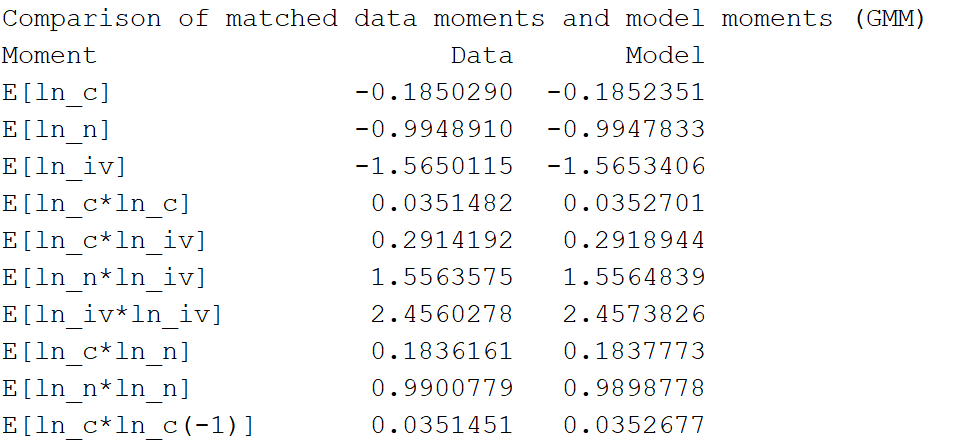
\includegraphics[width=8cm]{Figures/RBC_MoM_GMM_moments.png}
  \end{figure}
  \begin{witemize}
    \item Output is mostly similar to the one of \texttt{estimation}-command
    \item Results will be saved in \texttt{oo\_.mom}
    \item Results of J-test will also be displayed in the Command Window:\\
    
\includegraphics[width=8cm]{figures/J_test}
  \end{witemize}
\end{frame}

\begin{frame}{Dynare output: IRF matching}{\texttt{rbc\_irf\_matching.mod}}
\begin{figure}
    \centering
    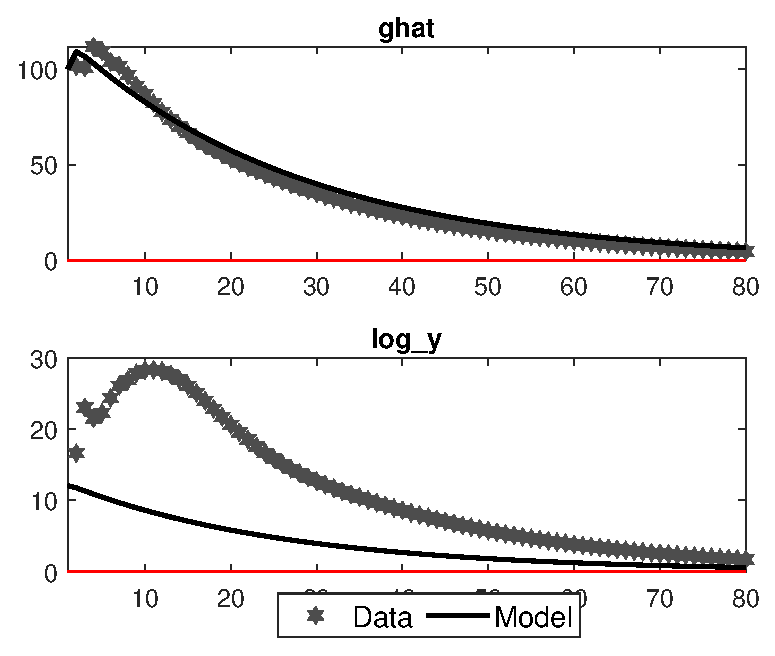
\includegraphics[width=7cm]{Example/IRF/rbc_irf_matching/graphs/rbc_irf_matching_matched_irf_eps_g1.eps}
\end{figure}
  \begin{witemize}
    \item IRF matching will also display graphical comparison of empirical and model IRFs
  \end{witemize}
\end{frame}